% !TeX spellcheck = en_US
\documentclass[10pt,a4paper]{article}
\usepackage[latin1]{inputenc}
\usepackage[T1]{fontenc}
\usepackage{amsmath}
\usepackage{amsfonts}
\usepackage{amssymb}
\usepackage{mathtools}
\usepackage{graphicx}
\usepackage{hyperref}
\hypersetup{
	colorlinks=true,
	linkcolor=blue,
	filecolor=magenta,
	urlcolor=gray
}

\usepackage{xcolor}
\usepackage{listings}

% Copyright 2017 Sergei Tikhomirov, MIT License
% https://github.com/s-tikhomirov/solidity-latex-highlighting/

\usepackage{listings, xcolor}

\definecolor{verylightgray}{rgb}{.97,.97,.97}

\lstdefinelanguage{Solidity}{
	keywords=[1]{anonymous, assembly, assert, balance, break, call, callcode, case, catch, class, constant, continue, constructor, contract, debugger, default, delegatecall, delete, do, else, emit, event, experimental, export, external, false, finally, for, function, gas, if, implements, import, in, indexed, instanceof, interface, internal, is, length, library, log0, log1, log2, log3, log4, memory, modifier, new, payable, pragma, private, protected, public, pure, push, require, return, returns, revert, selfdestruct, send, solidity, storage, struct, suicide, super, switch, then, this, throw, transfer, true, try, typeof, using, value, view, while, with, addmod, ecrecover, keccak256, mulmod, ripemd160, sha256, sha3}, % generic keywords including crypto operations
	keywordstyle=[1]\color{blue}\bfseries,
	keywords=[2]{address, bool, byte, bytes, bytes1, bytes2, bytes3, bytes4, bytes5, bytes6, bytes7, bytes8, bytes9, bytes10, bytes11, bytes12, bytes13, bytes14, bytes15, bytes16, bytes17, bytes18, bytes19, bytes20, bytes21, bytes22, bytes23, bytes24, bytes25, bytes26, bytes27, bytes28, bytes29, bytes30, bytes31, bytes32, enum, int, int8, int16, int24, int32, int40, int48, int56, int64, int72, int80, int88, int96, int104, int112, int120, int128, int136, int144, int152, int160, int168, int176, int184, int192, int200, int208, int216, int224, int232, int240, int248, int256, mapping, string, uint, uint8, uint16, uint24, uint32, uint40, uint48, uint56, uint64, uint72, uint80, uint88, uint96, uint104, uint112, uint120, uint128, uint136, uint144, uint152, uint160, uint168, uint176, uint184, uint192, uint200, uint208, uint216, uint224, uint232, uint240, uint248, uint256, var, void, ether, finney, szabo, wei, days, hours, minutes, seconds, weeks, years},	% types; money and time units
	keywordstyle=[2]\color{teal}\bfseries,
	keywords=[3]{block, blockhash, coinbase, difficulty, gaslimit, number, timestamp, msg, data, gas, sender, sig, value, now, tx, gasprice, origin},	% environment variables
	keywordstyle=[3]\color{violet}\bfseries,
	identifierstyle=\color{black},
	sensitive=false,
	comment=[l]{//},
	morecomment=[s]{/*}{*/},
	commentstyle=\color{gray}\ttfamily,
	stringstyle=\color{red}\ttfamily,
	morestring=[b]',
	morestring=[b]"
}

\lstset{
	language=Solidity,
	backgroundcolor=\color{verylightgray},
	extendedchars=true,
	basicstyle=\footnotesize\ttfamily,
	showstringspaces=false,
	showspaces=false,
	numbers=left,
	numberstyle=\footnotesize,
	numbersep=9pt,
	tabsize=2,
	breaklines=true,
	showtabs=false,
	captionpos=b
}


\lstdefinestyle{BashInputStyle}{
	language=bash,
	basicstyle=\small\sffamily,
	columns=fullflexible,
%	backgroundcolor=\color{yellow!20},
	linewidth=0.9\linewidth,
	xleftmargin=0.1\linewidth
}


\author{OCamlPro - Fabrice Le Fessant\footnote{Telegram: @fabrice\_dune} and Thomas Sibut-Pinote\footnote{Telegram: @ThomasSibutPinote} \\ \small{\url{https://github.com/OCamlPro/devex-18-zk-contest}}}
\title{Groth16 zk-SNARK Proof Verification on Freeton : Three Use Cases}
\date{}

\begin{document}
\maketitle

\newcommand{\zksnark}{zk-SNARK}
\newcommand{\zksnarks}{zk-SNARKs}


\section{Introduction}
\label{sec:intro}

\subsection{Description of the submission}
\label{subsec:description}

The present document is an official submission to the 18$^{\text{th}}$
contest\footnote{\url{https://devex.gov.freeton.org/proposal?proposalAddress=0\%3Ae6b65075478e7d412fdb0870452f30dfa8bf51272e28a3167abc5c5df6fd051d}}
of the DevEx governance: {\em Groth16 \zksnark{} Proof Verification Use
  Cases}. Although we accepted earlier to be part of the jury, we
understand that by submitting this document we waive our right to vote
in the present contest.

In this submission, we propose three different use cases for Groth16
\zksnark{} proofs on the FreeTON blockchain:
\begin{itemize}
\item (Section~\ref{section_sudoku}) Sudoku: \zksnarks{} are used to prove that the user has a solution
  to a given Sudoku problem, without providing the solutions to other
  users ;
\item (Section~\ref{section_euler})Project Euler: \zksnarks{} are used to prove that the user has found the solution to a math problem from the famous \url{https://projecteuler.net} website;
\item (Section~\ref{section_pincode})Pin-code reset of forgotten keys: \zksnarks{} are used to replace a
  pubkey when the user has lost his secret key.
\end{itemize}

We then show the contributions that we made for the Free TON community while working on
this contest (Section~\ref{sec:contributions}). Finally, we discuss the three paradigms of using \zksnarks{} that our examples showcase (Section~\ref{sec_three_paradigms}).

\subsection{General remarks}
\label{subsec:general_remarks}

\begin{description}
	\item[Code:] All our code comes with a README and tests. This document is provided as an overview of our use cases for \zksnarks{} on the Freeton blockchain but you can also directly plunge into the code. All our code is under the GPL license and is hosted at \url{https://github.com/OCamlPro/devex-18-zk-contest}.

	\item[Compilation time:] The long compilation time of the repository provided was a major obstacle in our progression. We would suggest trying to make it shorter for future contests.

	\item[Marshalling and memory corruption:] Because of a memory corruption error in the marshalling of the verification key, we were unable to do a full 9 by 9 Sudoku, restricting ourselves to 4 by 4. All our code is generic (it is generated from an OCaml program which takes as a parameter the value $n$ such that the Sudoku is $n^2$ by $n^2$). We were told that after the contest, a more robust marshalling library would be provided. In any case we would be glad to discuss this issue with the Nil foundation team to give users the full Sudoku experience! In the meantime, a 4 by 4 Sudoku is sufficient to get a sense of the dynamics of \zksnark-based Sudoku.

	\item[Keys on contracts: ] For all of our smart contracts, we provided, along with the verification key as needed by the \verb|vergroth16| instruction, the proving key (in a zipped) on the smart contract. This enables users to easily find it in order to generate their proofs. In case the contract deployer should decide to keep the possibility of changing the verification and proving keys of the problem(s), this also makes it easiest to follow changes before submitting a solution.

    \item[Separate submissions:] After deliberation, we decided to submit only one document rather than three separate submissions, in a spirit of coherence. We leave it to the appreciation of the jury whether this work deserves to be counted as several submissions.

	\item[Thanks:] We would like to thank @noam for his efforts and sportsmanship during the contest, and to the Nil foundation team for their answers to our various questions.
\end{description}










\section{A toy example: Sudoku}
\label{section_sudoku}

	\begin{figure}[!h]
	\centering
	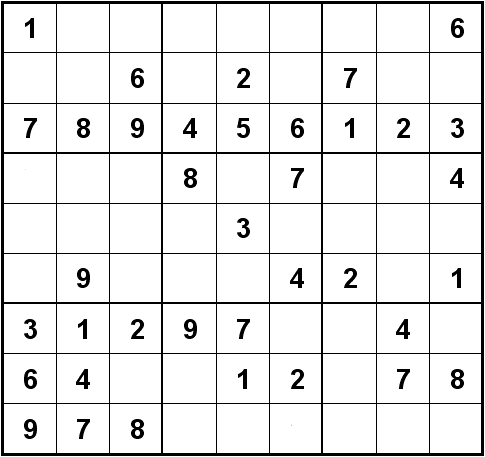
\includegraphics[width=0.6\textwidth]{Sudoku04}
	\caption{A Sudoku grid}
	\end{figure}


Let's start with our first toy use case. Suppose you want to set up a Sudoku problem for your students to solve, so that upon completion they receive some token. The issue is that once any student has solved it, the solution sits on the blockchain for all to see. All the other students can cheat by copying it, instead of doing the work by themselves, which defeats the whole purpose.

As mentioned in Section \ref{subsec:general_remarks}, we had to restrict ourselves to a 4 by 4 Sudoku grid, even though our code generator is generic in the grid size. This is because the marshalling function on the 9 by 9 code produced a memory corruption error.

\subsection{Mathematical encoding}
\label{subsec:math_enc}

\emph{Note: You may skip this section if you don't want to focus too much on the details on a first reading.}

Let $n^2$ be the size of a Sudoku grid (in our case, $n=2$ and $n^2 = 4$ is the length of a side of the Sudoku square).In the following, the variables $(x_{i,j})_{0 \leq i,j < n^2}$ denote the (secret) values of the solution of a given instance of a Sudoku. The variables $(f_{i,j})_{0 \leq i,j < n^2}$ denote the instance so that
\begin{equation}
f_{i,j} =
\begin{cases*}
0 & if \textrm{square $i$,$j$ is not fixed by the Sudoku instance}\\
\textrm{The value in square $i$,$j$ }        & otherwise
\end{cases*}
\end{equation}
The (well-known) constraints of a Sudoku are encoded by the following equations:
\[ \prod_{k=1}^{n^2} \left( x_{i,j} - k \right) = 0 \textrm{ for all $0 \leq i,j < n^2$} \]
and
\[ f_{i,j} x_{i,j} = f_{i,j}^2 \textrm{ for all $0 \leq i,j < n^2$}\]
and, for all $S$ set of indices representing a row, a column or a box as per the rules of Sudoku:
\[ \prod_{(i,j) \in S} x_{i,j} = \prod_{k=1}^{n^2} k = \left(n^2\right)! \; .\]


The first equations guarantee that the only permitted values for $x_{i,j}$ are the integers from $1$ through $n^2$, while the second force

\[ \forall 0 \leq i,j < n^2, f_{i,j} \neq 0 \implies x_{i,j} = f_{i,j}.\]

The last equation, by forcing the product of $n^2$ integers between 1 and $n^2$ to be equal to $\left(n^2\right)!$, forces every row, column and box to contain one and only one instance of the integers $1$ through $9$.

%One other advantage is that we don't need to implement the whole logic of the computation on the smart contract. For some size of Sudoku, this is probably worthwhile.

\subsection{Components}
\label{subsec:components}

This use case includes two different components:

\begin{description}
	\item[The cli:] it is a C++ program linked to the Blueprint \zksnarks{} library. It can be used in two different ways:
	\begin{itemize}
		\item To create the original proving and verification keys. This step is independent of any given Sudoku instance and should only be done once.
		\item To generate a proof given an instance and a solution. The instance is given as a text file such as

		\begin{verbatim}
			0000
			0000
			0000
			0001
		\end{verbatim}

		where $0$s denote free values. The solution should be a similar text files with no zeroes, such as

		\begin{verbatim}
			1234
			3412
			2143
			4321
		\end{verbatim}

		Note that if your solution is not correct, this step will fail.
	\end{itemize}
    \item[The Sudoku smart contract:] The main function of this smart contract is
    \begin{lstlisting}[language=Solidity]
    function submit(bytes proof)
        public view returns (bool res, string blob_str)
    \end{lstlisting}
    It will check the input proof against the verification key \lstinline[language=Solidity]|v_key| and the current instance \lstinline[language=Solidity]|m_instance|, both local to the contract. This instance is stored as an array of \lstinline[language=Solidity]|fixed_value|:
    \begin{lstlisting}[language=Solidity]
    struct fixed_value {
      uint8 i;
      uint8 j;
      uint8 value;
    }

    \end{lstlisting}
\end{description}

\subsection{Code}
\label{subsec:sudoku_code}

TODO: code du sudoku ici



\section{Project Euler}
\label{section_euler}

	\begin{figure}[!h]
	\centering
	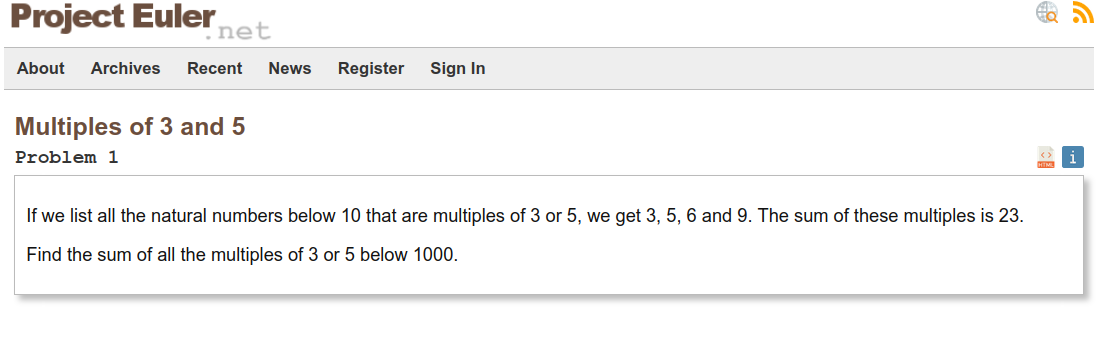
\includegraphics[width=\textwidth]{euler}
	\caption{The first Project Euler problem}
\end{figure}

The previous example is somewhat limited by the fact that Sudokus are easily solvable problems, either by hand or with a computer; they are not a realistic use case of \zksnarks{}\footnote{Although they hint at a possible use for \zksnarks{}: checking a result without implementing its full logic in Solidity may save precious storage and computations on the blockchain.}.

Let's keep the idea of a decentralized classroom. the famous website Project Euler\footnote{\url{https://projecteuler.net/}} offers math and programming problems of various difficulty to its users. It uses captchas to prevent brute force attempts at guessing the answer to a problem. The answers to problems are stored statically on its servers and the answers are checked against them. Can we make Project Euler decentralized? Using \zksnarks{}, we can prevent users from stealing others' solutions \textbf{and} from brute-forcing them, due to the cost of generating proofs.

The authentic first 50 problems from the Project Euler website\footnote{Solved by yours truly.}, are deployed and available on the Nil Foundation instance of the FreeTON blockchain.

\subsection{Brute-force protection}
\label{subsec:brute-force}

Project Euler is a gentlemen's competition. For example, competitors
are supposed to have found the answer using a program running at most
in one minute, but no mechanism enforces this. Still, some protections
are in place, partly to enforce the spirit of the competition, and
partly because of past abuse. For instance, a captcha system prevents
one from attempting many solutions in a row. We decided to emulate the
latter mechanism. If we simply gave a proving key to try and find the
actual solution to the problem, users might be tempted to try to build
a proof using every single integer until it works\footnote{We have
  noticed that although generating a correct proof may take time, an
  incorrect input is usually rejected in less than one
  second.}. Hence, the value they must find is actually
\[ \textrm{SHA256}^{1\,000\,000}\left(problem\_number | solution | nonce\right)\]
where the exponent denotes repeated application of the $\textrm{SHA256}$ hashing function, and `|` denotes the concatenation of strings. Note that this does not protect against replay attacks, which is why we also included a form of authentication described in Section~\ref{section_pincode}. This repeated application takes about 20 seconds on our laptops, which seems enough to discourage brute-force by all but the most determined cheaters.


\subsection{Components}
\label{subsec:euler_components}


This use case includes two different components:

\begin{description}
	\item[The cli:]
	\item[The EulerRoot TIP3-style contract:] Following the TIP3 conventions, this is the root contract to two types of leaves: EulerUser and EulerProblem. The EulerUser contract represents one user and the list of problems she has solved. The EulerProblem contract represents one problem and contains, among other things, the top ten leaderboard of the fastest solvers.
\end{description}

\section{Pin code reset for forgotten keys}
\label{section_pincode}

In this use case, we use \zksnarks{} to allow users to replace their
public keys in multisig wallets. The typical use is when a user has
lost the associated secret key, and is unable to sign/confirm any new
transaction. With our approach, the user first creates a recovery
contract, where a passphrase is associated to his public key. If he
needs to change his public key, he can use \zksnarks{} to associate a new
public key in his recovery contract, and tell multisig wallets to
safely replace his pubkey by the new one.

Compared to other approaches, this use can provide several
improvements:
\begin{itemize}
\item The user does not disclose his passphrase. Most other approaches
  (based on hashes for example) give an opportunity for
  man-in-the-middle attacks ;
\item As the user does not disclose his passphrase, the pubkey can be
  replaced several times ;
\item The user does not need to create the new public key ahead of
  time. Instead, he can create it when he has lost the former one,
  decreasing the likelihood of losing the associated secret key also ;
\end{itemize}

\subsection{Technical solution}

This use case includes 3 different components:
\begin{description}
\item[PinCode Client:] it is a C++ program linked to the Blueprint
  \zksnarks{} library. It can be used in two different ways:
  \begin{itemize}
  \item To create the initial circuit using the passphrase. The client
    should be called as:
\begin{verbatim}
pincode-client prepare "my pass phrase"
\end{verbatim}
   This will generate a file \lstinline{verifkey.hex} that can be used
   as an argument when deploying the \lstinline{PubkeyRecovery} smart
   contract, and a file \lstinline{provkey.hex} that can be used to
   create new witnesses ;
 \item To create a witness that the passphrase is known when providing
   a new public key. Because the witness contains the new public key,
   an attacker cannot intercept the message and replace it. The client
   should be called as:
\begin{verbatim}
pincode-client prove "my pass phrase" "PUBKEY_AS_HEX_NUMBER"
\end{verbatim}
  The command expects to find the file \lstinline{provkey.hex} and
  generates a file \lstinline{proof.hex} that should be submitted to
  the \lstinline{PubkeyRecovery} smart contract together with the new
  public key.
  \end{itemize}
\item[PubkeyRecovery smart contract:] This smart contract is a TIP-3
  contract, using the initial public key to verify its address. This
  contract is very simple. It contains:
  \begin{itemize}
  \item A constructor to set the circuit that will be used to verify
    that the passphrase is known when it is used ;
  \item An external function
    \lstinline{SetNewPubkey(bytes proof, uint256 pubkey)}
    to define the new public key, while providing a
    proof of knowledge of the passphrase ;
  \item An external function
    \lstinline{RecoverPubkey(address multisigaddr)}
    to call a multisig contract to update the
    corresponding custodian. The multisig contract will verify that
    the address is correct before replacing the public key ;
  \end{itemize}
\item[Modified Multisig Wallet:] This is a standard multisig wallet,
  modified to recognize addresses of \lstinline{PubkeyRecovery} smart
  contracts. They provide two additionnal functions:
  \begin{itemize}
  \item An external function
    \lstinline{SetPubkeyRecoveryCode(TvmCell code)}
    to define the code of the \lstinline{PubkeyRecovery} smart
    contract. Because the code hash is known, anybody can call this
    function with the correct code.
  \item An external function
    \lstinline{RecoverPubkey(uint256 oldkey, uint256 newkey)}
    that can only be called by a
    \lstinline{PubkeyRecovery} smart contract.
  \end{itemize}
\end{description}


\section{Contributions to the Free TON community}
\label{sec:contributions}

In the course of participating to this contest, we were led to refine
our in-house tools in order to more easily manipulate the Nil
Foundation forks of the Ton Virtual Machine (TVM), the TON Solidity
compiler and the TVM linker.

Our first contribution is a public Docker image containing the TONOS
SE compiled with \zksnarks{} support. The image is published as {\tt
  ocamlpro/nil-local-node} and is built from
\url{https://github.com/NilFoundation/tonos-se}.

Running it is simple:
\begin{verbatim}
docker run -d --name local-node -e USER_AGREEMENT=yes -p80:80 ocamlpro/nil-local-node
\end{verbatim}

Another way to use it is through our development tool {\tt ft}, a Free
TON Wallet designed for developers:
\url{https://github.com/OCamlPro/freeton_wallet}

For this contest, a set of improvements has been contributed to {\tt
  ft} to ease using it.

In particular:
\begin{itemize}
\item The interface has been improved to provide multiple levels of
  subcommands, making them easier to understand and to use ;
\item A new argument {\tt --image} is available with {\tt ft switch
  create} to specify the Docker image to use. This new argument is
  specially useful for our Docker image for NilFoundation TONOS SE.
\end{itemize}

As a consequence, a \zksnark-ready sandbox (local network) can be
installed by simply running:

\begin{lstlisting}[style=BashInputStyle]
ft switch create sandbox --image ocamlpro/nil-local-node
\end{lstlisting}

Now all commands from the \lstinline|ft| documentation will work, in
particular it will be easy to create accounts, deploy contracts, and
call them as seen in
\url{https://ocamlpro.github.io/freeton_wallet/sphinx/use-cases.html}.

The Docker image of \lstinline|ft| has been updated to use
NilFoundation tools
(\lstinline|solc|, \lstinline|tonos-cli|, \lstinline|tvm_linker|), it is
the easiest way to use \lstinline|ft| if you don't want to build
it. See the installation instruction at
(\url{https://ocamlpro.github.io/freeton_wallet/sphinx/install.html#using-docker}).

\section{Thoughts on three paradigms of \zksnarks{} on blockchains}
\label{sec_three_paradigms}
This contest has given us the opportunity to think harder about the categories of uses of \zksnarks{} on blockchains:
\begin{enumerate}
	\item Statically checking that someone has some information at their disposal(Euler case)
	\item Encoding a possibly complex computation in a circuit and challenging a user with an instance of that computation (Sudoku case)
	\item Using the \zksnark{} as an extension of the blockchain protocol itself (pincode, anonymous transactions, voting protocols)
\end{enumerate}

Of course, the boundaries between these categories may be blurred, but still they are meaningful. The point of the first category is that the data whose existence we are verifying is inert, static, it was chosen by the verifier according to some human meaning which is completely meaningless to the contract or the blockchain. In the second category, the value whose existence we are verifying has a computational (i.e. mathematical, see Section~\ref{subsec:math_enc}) meaning, and though this computational meaning\footnote{Of course, the answers to the Project Euler problems do have computational meaning ultimately, but no program is provided to encode the problem or check the solution. This computational meaning is inferred from the english description of the problem by the problem solver.} is not present on the blockchain itself, it is implicitly present in the verification key. Finally, the third category consists in the verification of data which has blockchain-protocol-level computational meaning (such as a public key). The privacy aspect of \zksnarks{}, which is of course the whole point, had initially hidden these distinctions from us.

In category 1, the main advantage of \zksnarks{} is to not spoil the fun for other competitors. One must protect oneself from replay attacks (re-using the same zero-knowledge proof as some other competitor in order to pretend one has solved the problem) and brute-forcing the answer.

In category 2, the point is to guarantee some mathematical properties of a wide range of submitted solutions to a given problem of a known computational nature, when not all of possible instances may be computed in advance. The \emph{zero-knowledge} part may or may not be important, but the \emph{succinct} part may well save some gas for cost-heavy verifications.

In category 3, the zero-knowledge part plays a crucial part in preventing man-in-the-middle attacks for security-critical operations such as changing a lost public key in a wallet, or sending an anonymous amount of tokens to an anonymous recipient, or voting without revealing one's ballot.

These three categories may be combined in several ways depending on the purpose.

\end{document}
